\begin{figure}[htbp]
\centering
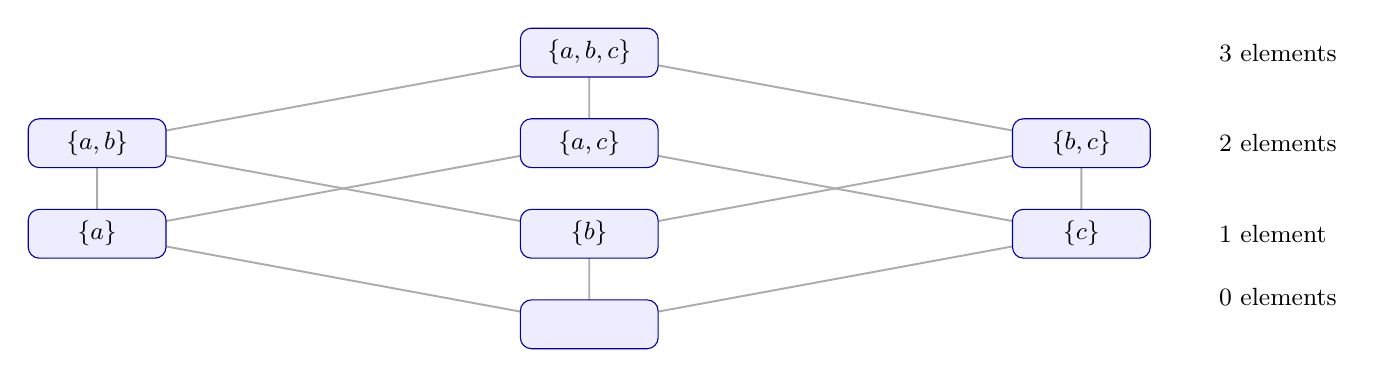
\begin{tikzpicture}[x=1.25cm,y=1cm]
    \tikzset{setnode/.style={draw=blue!65!black,fill=blue!7,rounded corners,minimum width=1.75cm,minimum height=0.62cm,inner sep=3pt,font=\small}}
    \draw[gray!65,line width=0.7pt] (5,0) -- (0,1.15) (5,0) -- (5,1.15) (5,0) -- (10,1.15);
    \draw[gray!65,line width=0.7pt] (0,1.15) -- (0,2.3) (0,1.15) -- (5,2.3);
    \draw[gray!65,line width=0.7pt] (5,1.15) -- (0,2.3) (5,1.15) -- (10,2.3);
    \draw[gray!65,line width=0.7pt] (10,1.15) -- (5,2.3) (10,1.15) -- (10,2.3);
    \draw[gray!65,line width=0.7pt] (0,2.3) -- (5,3.45) (5,2.3) -- (5,3.45) (10,2.3) -- (5,3.45);

    \node[setnode] at (5,0) {$\varnothing$};
    \node[setnode] at (0,1.15) {$\{a\}$};
    \node[setnode] at (5,1.15) {$\{b\}$};
    \node[setnode] at (10,1.15) {$\{c\}$};
    \node[setnode] at (0,2.3) {$\{a,b\}$};
    \node[setnode] at (5,2.3) {$\{a,c\}$};
    \node[setnode] at (10,2.3) {$\{b,c\}$};
    \node[setnode] at (5,3.45) {$\{a,b,c\}$};

    \node[anchor=west,font=\small] at (11.3,0.35) {$0$ elements};
    \node[anchor=west,font=\small] at (11.3,1.15) {$1$ element};
    \node[anchor=west,font=\small] at (11.3,2.3) {$2$ elements};
    \node[anchor=west,font=\small] at (11.3,3.45) {$3$ elements};
\end{tikzpicture}
\caption{The power set $\mathcal{P}(\{a,b,c\})$ ordered by inclusion. Each edge adds one element, so every upward path follows a chain of subsets.}
\label{fig:power-set-lattice}
\end{figure}